\documentclass{beamer}
\usepackage{beamerthemesplit} % new

\usepackage[utf8]{inputenc}
\usepackage[utf8]{inputenc}
\usepackage{tikz}

\newcommand{\roundpic}[4][]{
  \tikz\node [circle, minimum width = #2,
    path picture = {
      \node [#1] at (path picture bounding box.center) {
        \includegraphics[width=#3]{#4}};
    }] {};}

\usepackage{graphicx,wrapfig,lipsum}
\usepackage{multicol}

\usepackage{tcolorbox}


\begin{document}
\title{MY-NEIGH}
\author{BDBI\_2019\_GR\_04}
\date{\today}

\frame{\titlepage}

\frame{\frametitle{Table of contents}\tableofcontents}


\section{Team Members}


    
\frame{\frametitle{Team}
  \begin{itemize}
    \item MARTA IBÁÑEZ 
    \item JUDIT CAMPS   
    \item AINA MONTALBAN 
  \end{itemize}
  \vspace{1cm}
  \hspace{2cm}
 \roundpic[xshift=-0.03cm,yshift=-0.03cm]{2cm}{2cm}{images/marta.png}
   \hspace{0.5cm}
 \roundpic[xshift=-0.03cm,yshift=-0.03cm]{2cm}{2cm}{images/judit.JPG}
    \hspace{0.5cm}
  \roundpic[xshift=-0.03cm,yshift=-0.03cm]{2cm}{2cm}{images/aina.JPG}


}


\section{Trello}
\subsection{Trello Tasks}
\frame{\frametitle{Trello}
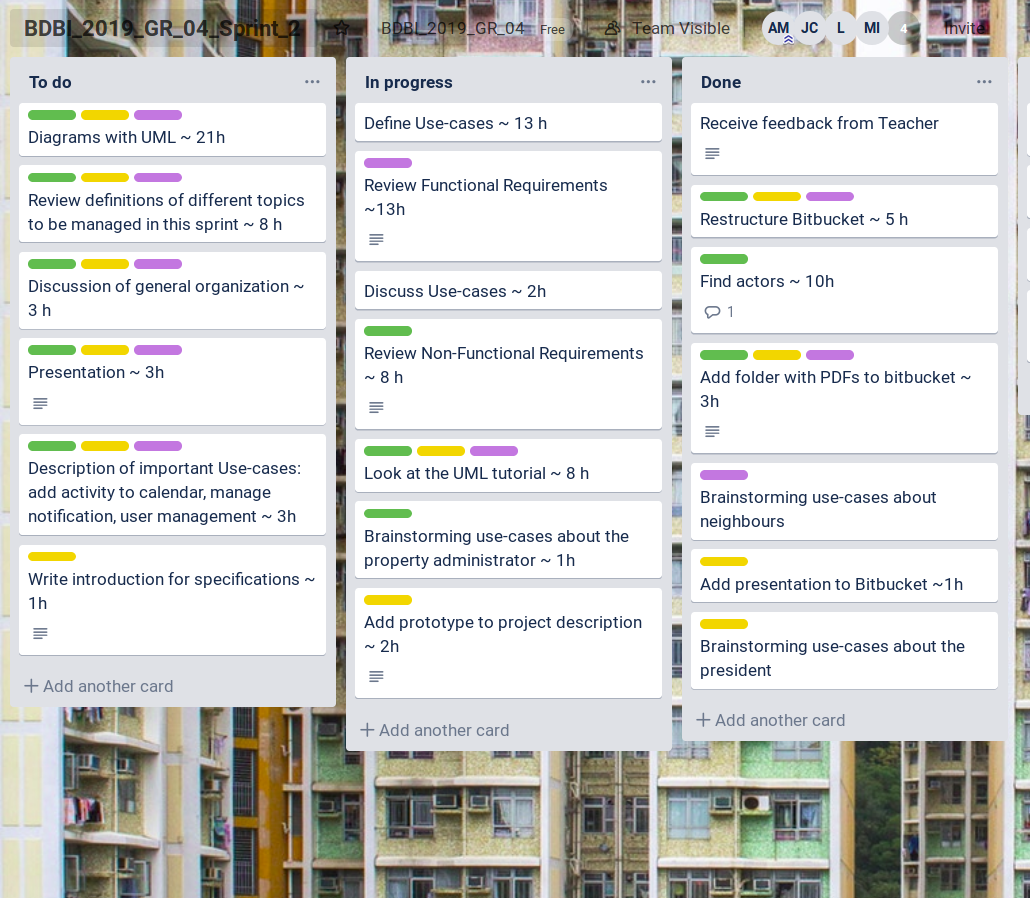
\includegraphics[width=6cm, height=5cm]{images/trello-s2.png}
}
\section{Trello}
\subsection{Trello Description}
\frame{\frametitle{Trello}
Example of description:
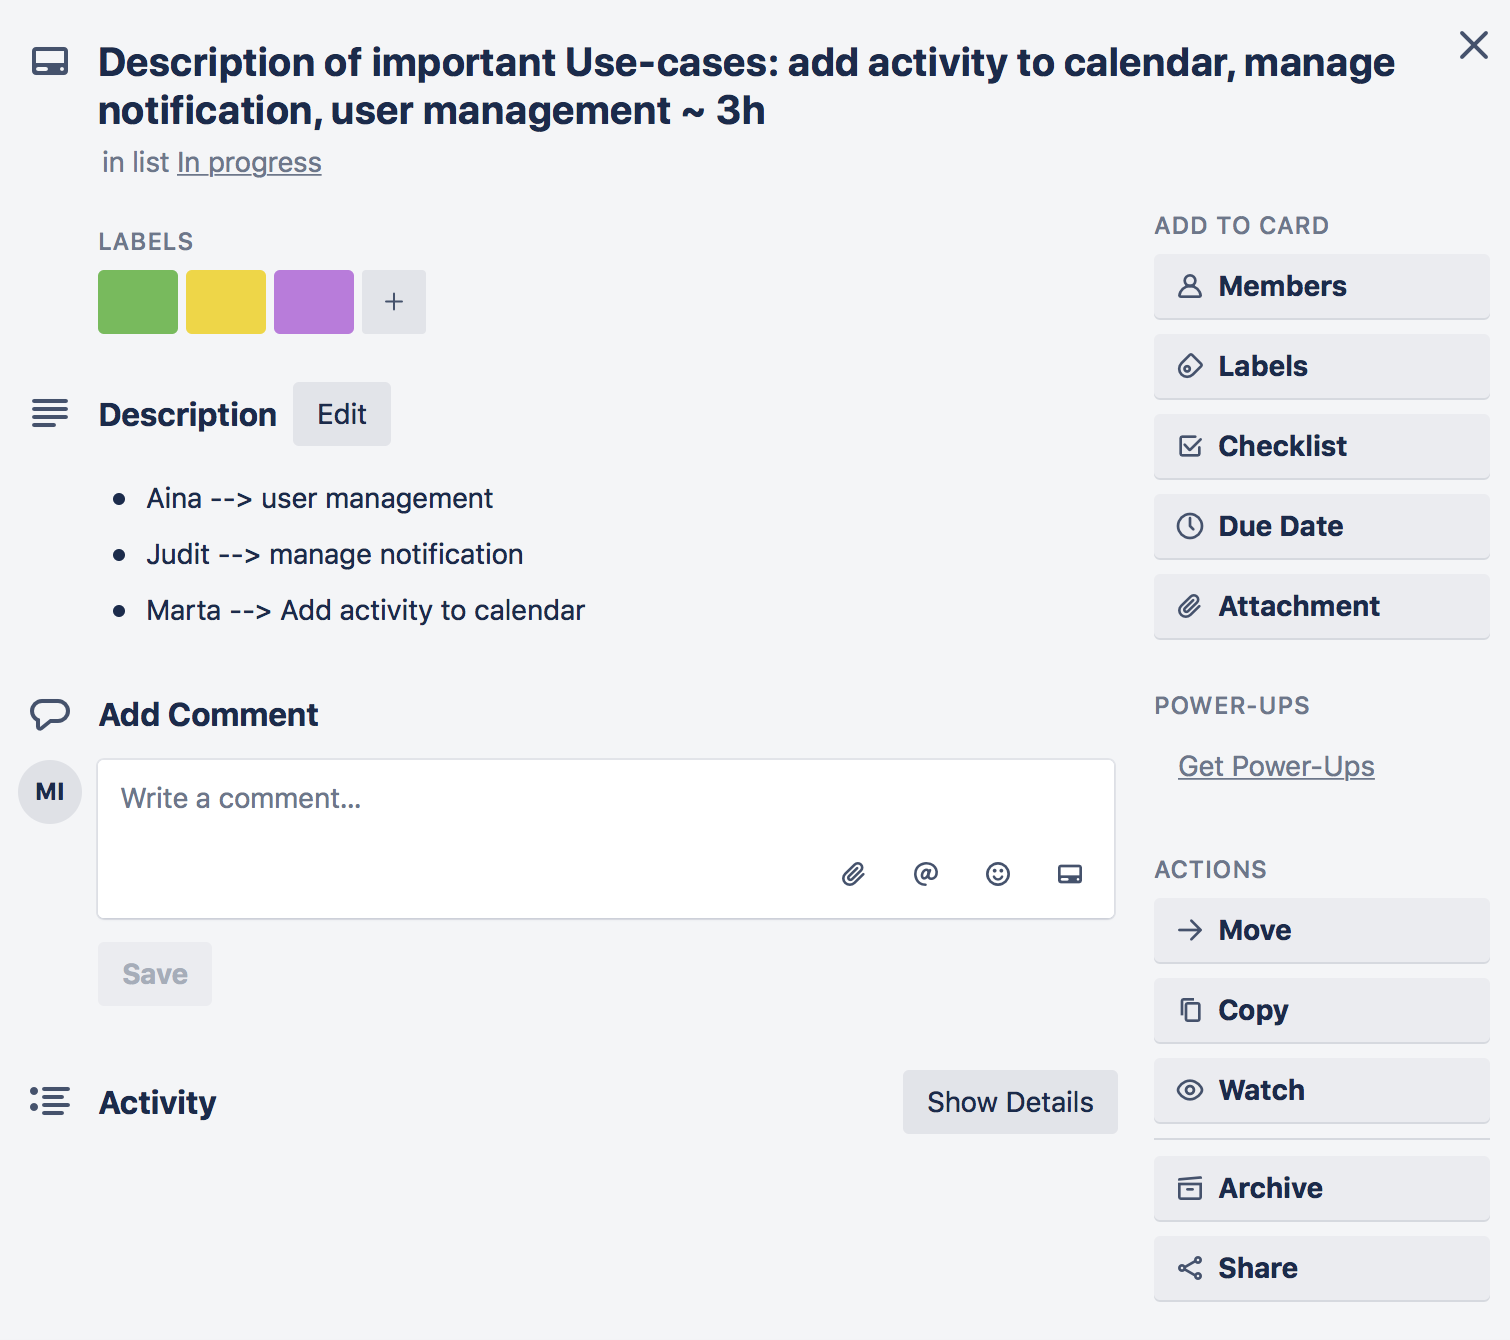
\includegraphics[width=5cm, height=5cm]{Trello_descr.png}
}
\frame{\frametitle{Plan}
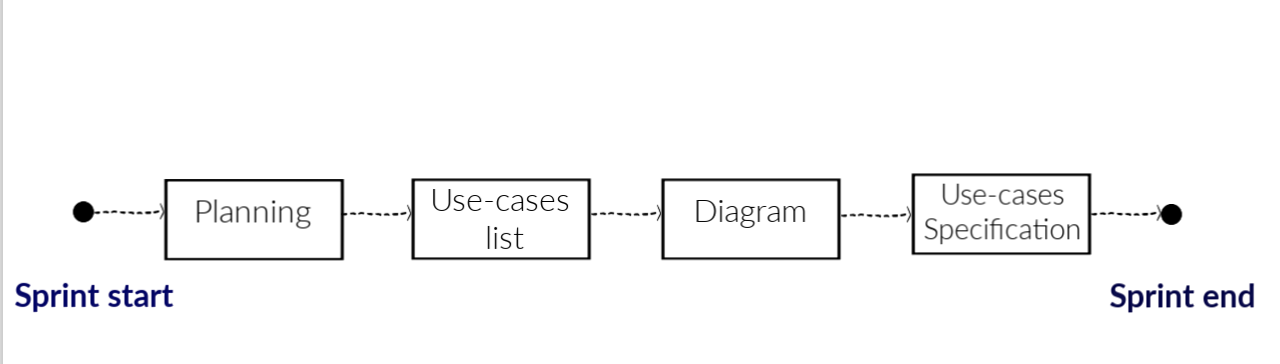
\includegraphics[width=\textwidth]{Plan.png}
}
\frame{\frametitle{Done}
\begin{itemize}
    \item Planning of the sprint
    \item Actors
    \item Look for use-cases
    \item Specification of use-cases
\end{itemize}
}

\section{Bitbucket}
\frame{\frametitle{Bitbucket}
%Last sprint
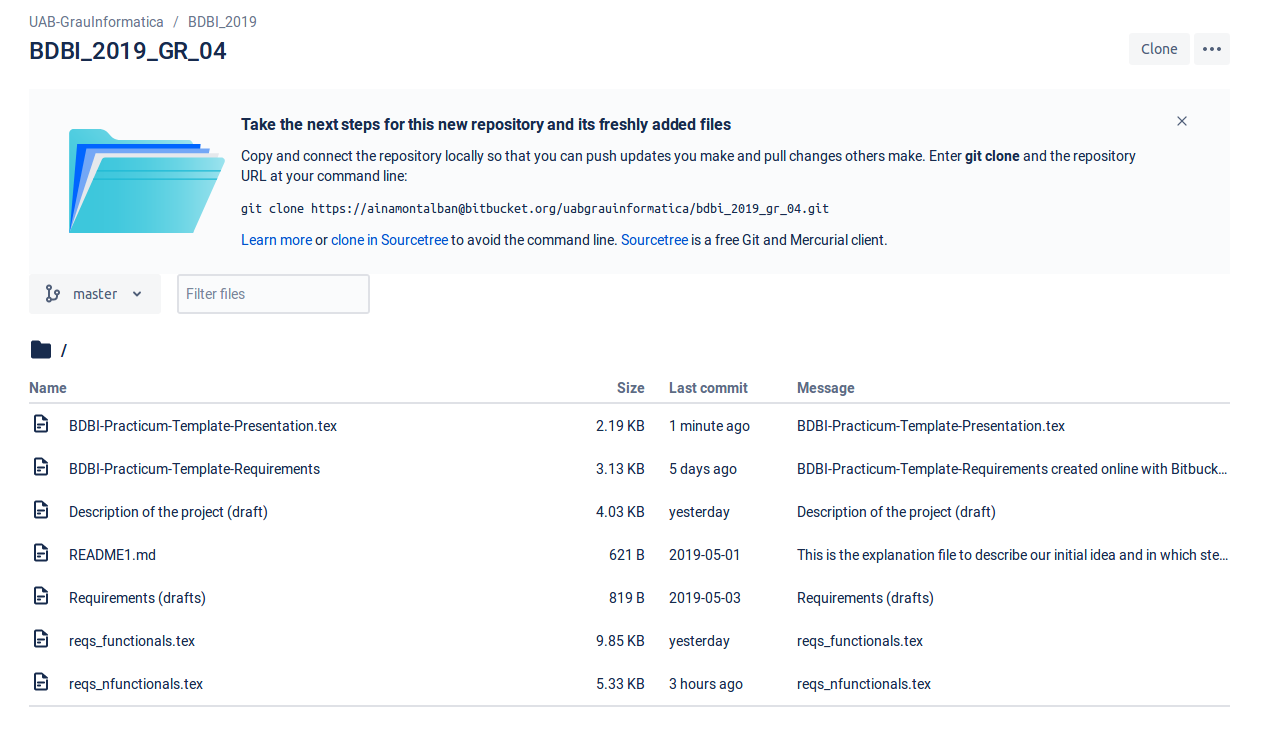
\includegraphics[width=9cm, height=6cm]{bitbuck.png}
}

%Current sprint
\frame{\frametitle{Bitbucket}
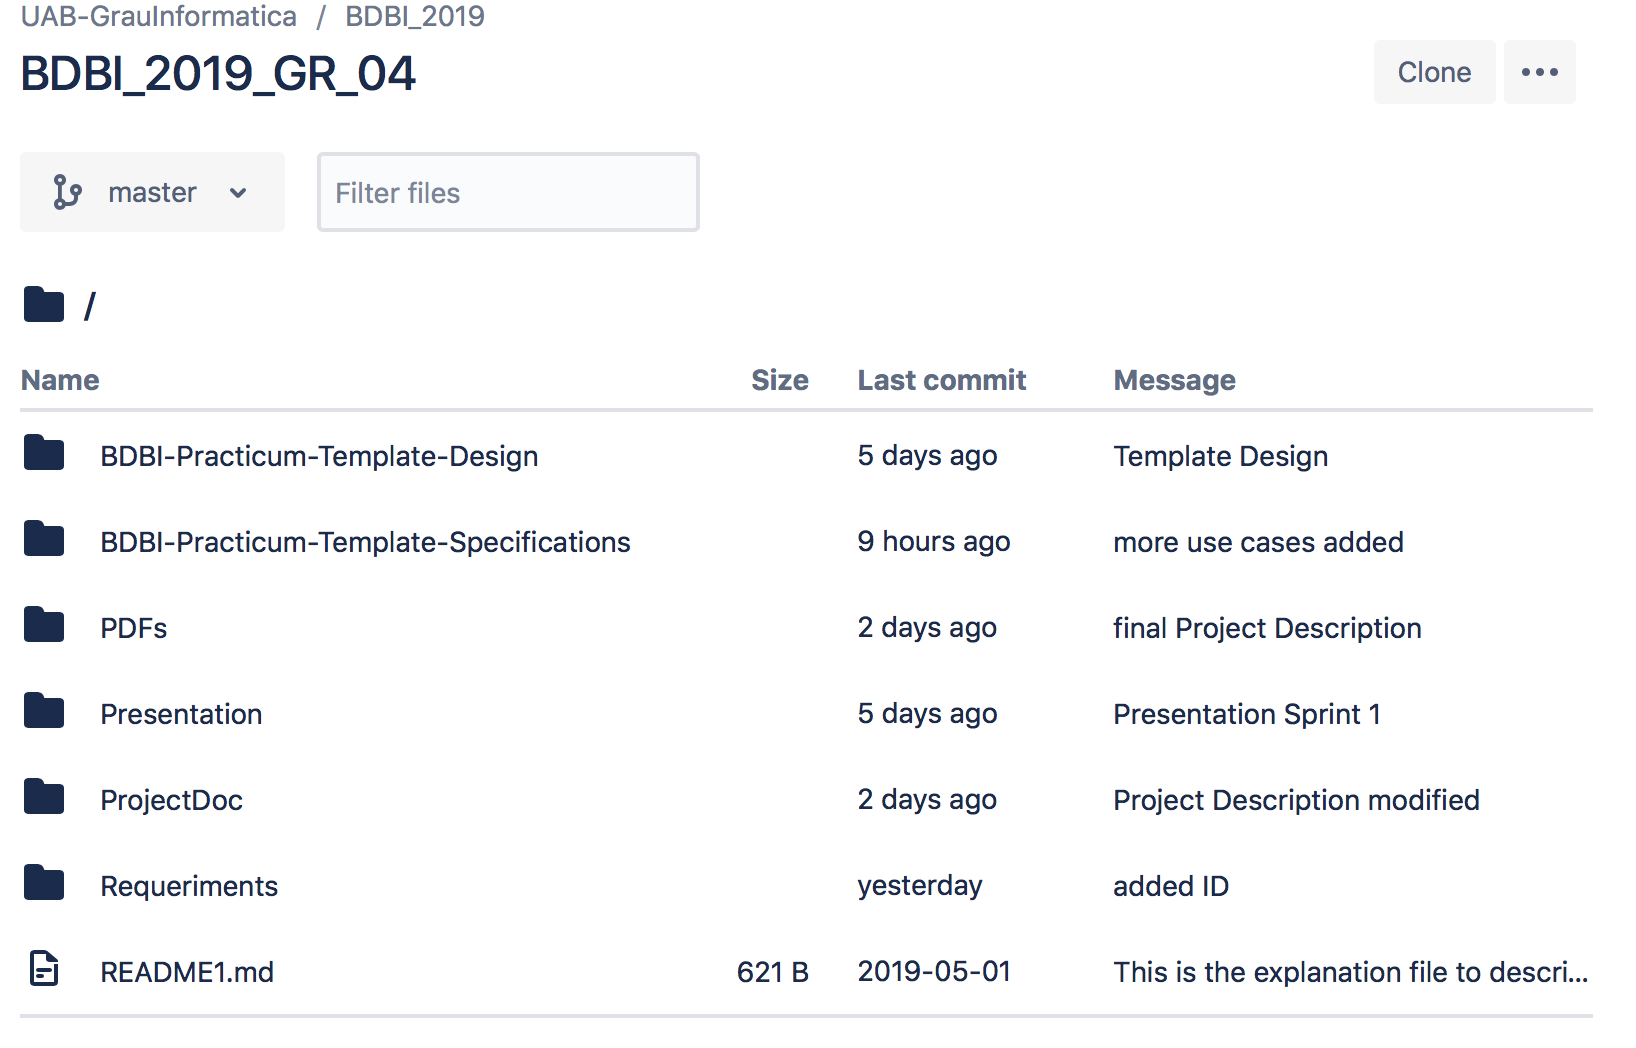
\includegraphics[width=9cm, height=6cm]{Bitbucket.png}
}


\section{Actors}
\frame{\frametitle{Actors}
\begin{itemize}
    \item Neighbour
    \item President
    \item Property Administrator
    \item App Administrator
\end{itemize}
}

\section{Use-case Diagram}
\frame{\frametitle{Use-case Diagram}
}

\section{Use-case Specifications}
\frame{\frametitle{Use-case Specifications}
Specification of:
\begin{itemize}
    \item Add activity to calendar
    \item Manage notification
    \item User management 
\end{itemize}
}

%Add activity to calendar here
\subsection{Add activity to calendar}
\frame{\frametitle{Use-case Specifications}
}

%Manage notification here
\subsection{Manage notification}
\frame{\frametitle{Use-case Specifications}
}

%User management here
\subsection{User management}
\frame{\frametitle{Use-case Specifications}
}



\section{Conclusions}
\frame{\frametitle{Conclusions}
\begin{itemize}
    \item A lot of use-cases
    \item Improvement of Bitbucket, Trello, Latex 
    \item Clearer idea of our application
    \item 
\end{itemize}
}

\end{document}
